\chapter*{FUGE - FUzzy Genetic Engine}
\section*{Evolution of a classifier based on fuzzy systems for the detection of arrhythmia}

Le set de données ``arrhythmia'' contient des informations pertinantes pour détecter une arythmie chez 452 sujets. Le set contient 279 entrées (ou features) et une classe de sortie qui indique si l'échantillons appartient à une personne qui souffre d'arythmie ou non.

Nous allons premièrement tester l'outil FUGE avec le set de données que nous avons à disposition. Nous changeons différents paramètres pour trouver les valeurs qui donnent les meilleurs résultats sur un faible nombre de générations, ici 100. Ces tests par tatonnement sont visibles dans le tableau \ref{searchparameters}.

\begin{table}[h!]
   \centering
   \begin{tabular}{|c|c|c|c|c|c|c|c|}
      \hline
      Test & Pop & Elite Pop & Crossover & Mutation & Bit Mutation & Size system weight & Fitness\\
      \hline
      1 & 200 & - & - & - & - & - & 0.73\\
      \rowcolor{very-light-gray}
      2 & 250 & - & - & - & - & - & 0.75\\
      3 & 300 & - & - & - & - & - & 0.74\\
      \hline
      4 & 250 & 3 & - & - & - & - & 0.71\\
      \rowcolor{very-light-gray}
      5 & 250 & 5 & - & - & - & - & 0.75\\
      6 & 250 & 7 & - & - & - & - & 0.74\\
      7 & 250 & 10 & - & - & - & - & 0.71\\
      \hline
      8 & 250 & 5 & 0.5 & - & - & - & 0.72\\
      \rowcolor{very-light-gray}
      9 & 250 & 5 & 0.9 & - & - & - & 0.75\\
      10 & 250 & 5 & 1 & - & - & - & 0.52\\
      \hline
      11 & 250 & 5 & 0.9 & 0.1 & - & - & 0.72\\
      \rowcolor{very-light-gray}
      12 & 250 & 5 & 0.9 & 0.15 & - & - & 0.75\\
      13 & 250 & 5 & 0.9 & 0.4 & - & - & 0.72\\
      \hline
      14 & 250 & 5 & 0.9 & 0.15 & 0.01 & - & 0.7505\\
      \rowcolor{very-light-gray}
      15 & 250 & 5 & 0.9 & 0.15 & 0.025 & - & 0.7517\\
      16 & 250 & 5 & 0.9 & 0.15 & 0.05 & - & 0.7502\\
      \hline
      \rowcolor{very-light-gray}
      17 & 250 & 5 & 0.9 & 0.15 & 0.025 & 0 & 0.7519\\
      18 & 250 & 5 & 0.9 & 0.15 & 0.025 & 0.01 & 0.738\\
      19 & 250 & 5 & 0.9 & 0.15 & 0.025 & 0.1 & 0.70\\
      \hline
   \end{tabular}
   \caption{\label{searchparameters} Recherche des meilleurs paramètres}
\end{table}



Maintenant que nous avons trouvé de bons paramètres qui sont ceux illustrés à la figure \ref{parameters}, nous pouvons faire des tests sur un plus grand nombre de générations.


\begin{figure}[h]
  \centering
    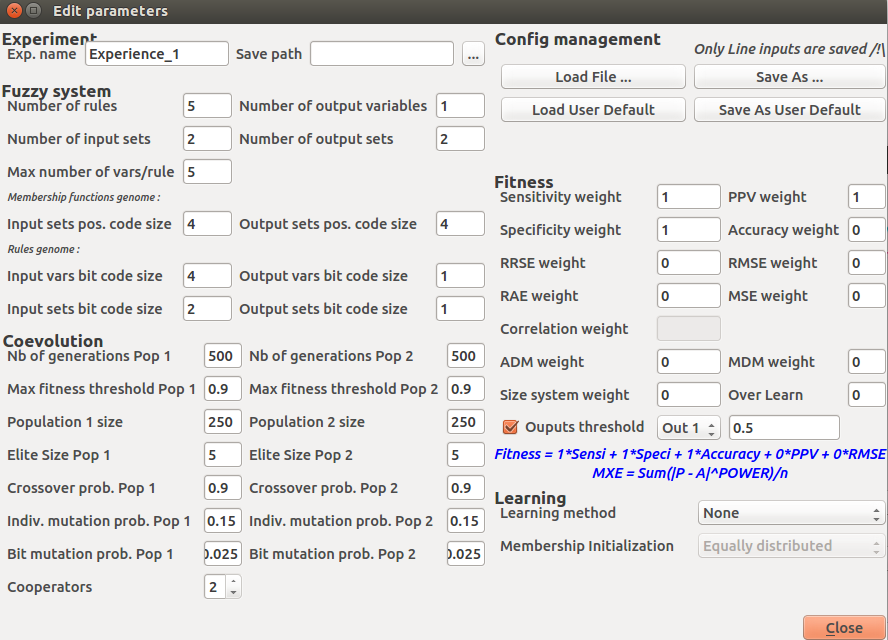
\includegraphics[width=0.8\linewidth]{img/values.png}
  \caption{Paramètres idéaux trouvés}
  \label{parameters}
\end{figure}

Nous avons fait trois tests avec 500 générations pour être sûr que la valeur de fitness ne change plus. Les résultats se trouvent dans la table \ref{resulttab500}. Nous avons donc une moyenne de valeur de fitness qui se trouve à 78.15\%.


\begin{table}[h!]
   \centering
   \begin{tabular}{|c|c|c|c|c|}
      \hline
      Test & Valeur de fitness \\
      \hline
      1 & 0.7920 \\
      2 & 0.7734 \\
      3 & 0.7791 \\
      \hline
      moyenne & 0.7815 \\
      \hline
   \end{tabular}
   \caption{\label{resulttab500} Valeurs de fitness trouvées sur 500 générations}
\end{table}

% Code integration example
%\begin{lstlisting}[language=bash]
%  sudo apt-get update
%  sudo apt-get install drupal7
%\end{lstlisting}

% Image integration example
%\begin{figure}[h]
%  \centering
%    \includegraphics[width=1\linewidth]{img/drupalFirstPage.png}
%  \caption{Page d'accueil du site créé avec Drupal sur une instance EC2}
%  \label{drupalfirstpage}
%\end{figure}

% Image side-by-side
%\begin{figure}[h!]
%    \centering
%    \begin{tabular}{cccc}
%      \includegraphics[width=.14\linewidth]{randomTree_n5.png} &
%      \includegraphics[width=.22\linewidth]{randomTree_n10.png} &
%      \includegraphics[width=.22\linewidth]{randomTree_n15.png} \\
%      (a) & (b) & (c)\\
%    \end{tabular}
%    \caption{Arbres aléatoires où (a) n=5 (b) n=10 (c) n=15
%    \label{randomTrees}}
%\end{figure}
